\documentclass[11pt]{scrartcl}
\usepackage{answers}
\Newassociation{sketch}{hintitem}{hints}
\renewcommand{\solutionextension}{out}
\usepackage[UTF8]{ctex}
\usepackage{amsfonts}
\usepackage[sexy]{evanjim}
\usepackage{graphicx}
\usepackage{subfigure}


\title{谱聚类实现}
\author{王晨旭\quad 1120223433}     %姓名 学号
\date{2024年7月2日}            % 上课日期

\begin{document}
\maketitle
\section{引言}                                               
谱聚类作为一种基于图论和谱图理论的聚类方法,在处理复杂数据结构和非线性关系时显示出了优越性。本文旨在探讨谱聚类的基本原理、实现步骤以及其在不同数据集上的表现。首先,我们将介绍构建无向图所需的基本概念,如图的定义、邻接矩阵和度数矩阵的作用。随后,我们将详细讨论拉普拉斯矩阵及其在谱聚类中的关键角色,包括其性质和应用。最后,我们将展示谱聚类算法的实现步骤,并通过实验和比较分析其与传统聚类方法的差异和优劣。通过本文的研究,读者将能够深入了解谱聚类在数据分析和模式识别中的应用及其算法优化的关键因素。


\section{前置知识}
本章节我们主要会讲述一些谱分析中常用的概念与对应的性质,包括图的定义,如何将原始数据构建为无向图,以及聚类的基本定义。
\subsection{图基本概念}
\begin{definition}[图的定义]
对于一个图$G=(V,E)$,其中$V=(v_1,...,v_n)$为图$G$的顶点集(这里$n$为顶点的数量),$E$为边的集合
\end{definition}                


\begin{definition}[邻接矩阵$W$]
在图$G=(V,E)$中,对于有边相连的两个顶点$v_i,v_j$,其对应的权值$w_{ij}>0$,否则$w_{ij}=0$.通常我们考虑图$G$为无向图,因此$w_{ij}=w_{ji}$,$W$为对称矩阵。
\end{definition}

\begin{definition}[度数矩阵D]
在图$G=(V,E)$中,我们定义顶点的度为与其他顶点对应的权值之和
$$
d_i=\sum_{j=1}^n w_{ij}
$$
利用每个顶点的度的定义,我们可以得到$n\times n$的度数矩阵$D$,且$D$中除主对角线元素均为0.
$$
D=\\diag\{d_1,...,d_n\}
$$
\end{definition}





\subsection{图的构建}
对于一个给定的数据集合$X=\{x_1,...,x_n\}$,其中$x_i\in R^k(k\ge1)$,我们无法直接得到这些数据点在图上的关系,因此我们需要利用一些方式将它们构建为一个图。常见的用于构建图(的邻接矩阵)的方式有以下三种:
\begin{enumerate}
\item $\varepsilon$邻近法:设定一个距离的阈值$\varepsilon$,然后利用欧式距离$s_{ij}$去度量任意两个顶点$x_i,x_j$的距离,其中
$$
s_{ij}=\sum_{l=1}^k (x_i(l)-x_j(l))^2
$$
根据$s_{ij}$与$\varepsilon$的大小来定义邻接矩阵W
$$
W=\left\{
\begin{aligned}
0&&s_{ij}>\varepsilon\\
\varepsilon &&s_{ij}<\varepsilon
\end{aligned}
\right.
$$
但是这样的度量方式实际上是极其不准确的,因为所有的权值均为$\varepsilon$或0,无法表现出数据间的相近程度,因此通常我们不会考虑使用该方式。


\item $KNN$邻近法:对于任意一个数据点$x_i$而言,我们利用$KNN$得到与之最相近的$l$个数据点$x_{i1},...,x_{il}$,并设置
$$
w_{ij}=\left\{
\begin{aligned}
0&&j \not\in \{x_{i1}...,x_{il}\}\\
exp(-\frac{s_{ij}}{2\sigma^2}) &&j\in \{x_{i1}...,x_{il}\}
\end{aligned}
\right.
$$
其中$\sigma$为常数。为了保证邻接矩阵$W$的对称性,我们对上述要求进行加强。当且仅当$x_i,x_j$互为$l$近邻点时,$w_{ij}>0$

\item 全连接法:利用核函数定义邻接矩阵的权值,如
$$
w_{ij}=exp(-\frac{s_{ij}}{2\sigma^2})
$$
其中$\sigma$为常数。这里根据不同核函数的选取,构建出的邻接矩阵会有很大的差异。并且该方法构建的邻接矩阵中,所有的权值均大于0.
\end{enumerate}


\subsection{拉普拉斯矩阵与相关性质}
拉普拉斯矩阵是谱图理论中较为重要的一个矩阵,对拉普拉斯矩阵的分析可以揭示大量图上的性质。以下我们将简单介绍拉普拉斯矩阵的性质,以及其在谱聚类领域的相关应用。
\begin{definition}[拉普拉斯矩阵$L$]
在图$G=(V,E)$中,定义其拉普拉斯矩阵为
$$
L=D-W
$$
\end{definition}
拉普拉斯矩阵具有丰富的性质,以下简单介绍部分与谱聚类相关的性质定理。为了便于读者阅读,我们将定理的证明放置于附录部分,并配以详实的解释说明。

\begin{theorem}
拉普拉斯矩阵$L$为对称半正定矩阵
\end{theorem}
其实我们可以由邻接矩阵$W$与度数矩阵$D$均为对称矩阵直接得到,当然也可通过如下证明得到:
对于任意$x\in R^n$,只需要证明$x^T L x\ge 0$即可


\begin{equation}
\begin{aligned}
x^T L x &= x^T D x-x^T W x\\
&=\sum_{i=1}^n d_i x_i^2-\sum_{e_{ij}\in E}w_{ij}x_ix_j\\
&=\frac{1}{2}\sum_{e_{ij}\in E}w_{ij}(x_i-x_j)^2
\end{aligned}
\end{equation}

\begin{theorem}
拉普拉斯矩阵$L$有$n$个非负的特征值,并且$0\le \lambda_1\le...\le\lambda_n$
\end{theorem}
我们将在附录中详细说明该定理的证明



\subsection{聚类}
聚类(Clustering)是一种将数据集中的对象分成多个簇或组的过程,使得同一簇内的对象在某种意义上比其他簇内的对象更为相似。常见的聚类方式包括k-means,层次聚类等,本章节我们主要集中与讨论谱聚类的优化目标与其背后的基本原理。
\begin{definition}[图的分割]
对于无向图$G=(V,E)$中,我们定义$A_1,...,A_k$为图$G$的一个k分割,当且仅当满足
$$
\forall i\not =j,A_i\cap A_j=\varnothing 
$$
$$
\cup_{i=1}^k A_i=V
$$
\end{definition}

\begin{definition}[切图权重]
设$A,B$为图$G=(V,E)$的两个子图,定义其切图权重为

$$
W(A,B):=\sum_{i \in A,j \in B} w_{ij}
$$
更为一般地,对于图$G$的一个k分割$A_1,...,A_k$,定义切图为
$$
cut(A_1,...,A_n)=\frac{1}{2}\sum_{i=1}^k W(A_i,\overline{A_i})
$$
其中$\overline{A_i}$为$A_i$的补集
\end{definition}
回顾聚类的基本原理,我们希望将相似的数据归为一个聚类簇,并且将不同的数据点分开。这样的性质在图上的表示为,对于一个k分割$A_1,...,A_k$,我们希望$A_i$内部的边(权重和)尽量地多,并且$A_i,A_j$之间的边(权重和)尽量地少。实际上我们只需要优化$cut(A_1,...,A_k)$,使得它最小即可。\\
但这样其实有一个问题,我们很难避免一些极端的情况,如某一个分割$A_i$中仅包含极为少数的点,这对于我们而言是不太良好的。因此我们对$cut(A_1,...,A_k)$进行如下加强:

\begin{definition}[Ratiocut]
对于图$G=(V,E)$的一个分割$A_1,...A_k$,我们同时希望$cut(A_1,...,A_k)$尽量小,并且$A_i$中点尽量多,因此可以利用$Ratiocut(A_1,...,A_k)$代替$cut(A_1,...,A_k)$
$$
Ratiocut(A_1,...,A_k)=\frac{1}{2}\sum_{i=1}^k \frac{W(A_i,\overline{A_i})}{|A_i|}
$$
当然我们也存在另一种加强方式,即$Ncut$
$$
Ncut(A_1,...,A_k)=\frac{1}{2}\sum_{i=1}^k \frac{W(A_i,\overline{A_i})}{vol(A_i)}
$$
其中$vol(A_i)=\sum_{j \in A_i} d_i$
\end{definition}
显然在图$G$为正则图时,$Ratiocut$与$Ncut$是等价的。这里我们不妨以$Ratiocut$为例进行接下来的讨论。\\

目前我们难以将$Ratiocut$与代数手段直接结合,因此我们考虑利用rounding操作。这是一个谱分析中的常用方法,本质上是将一个实数域上的规划问题转化为一个0/1规划问题(这里与本节内容无关,便不过多解释)。\\
具体的rounding操作如下:\\
对于每一个$A_i$,我们设置$y_i\in R^n$,并且
$$
y_i(j)=\left\{
\begin{aligned}
0&&v_j \not \in A_i \\
\frac{1}{\sqrt{|A_j|}}&&v_j \in A_i
\end{aligned}
\right.
$$
设$L=(l_{ij})$为图$G$的拉普拉斯矩阵,$W=(w_{ij})$为图$G$的邻接矩阵,那么

\begin{equation}
\begin{aligned}
y_i^T L y_i 
&=\sum_{e_{jk}\in E} y_i(j)y_i(k)l_ij\\
&=\sum_{e_{ij}\in E} w_ij(y_i(j)-y_i(k))^2\\
&=\frac{cut(A_i,\overline{A_i})}{|A_i|}\\
&Ratiocut(A_i,\overline{A_i})
\end{aligned}
\end{equation}

令$y_1,...,y_k$构成矩阵$Y$,我们可知:
$$
Ratiocut(A_1,...,A_k)=\sum_{i=1}^k y_i^T L Y_i=tr(Y^T LY)
$$
我们注意到$Y^TDT=I$,因此令$Y=D^{-\frac{1}{2}}$Z,其中$D$为图$G$的度数矩阵,那么只需要使得
$$
\min{tr(Z^T D^{-\frac12} L D^{-\frac12} Z)},Z^TZ=I
$$
即可。我们称$\mathscr{L}=D^{-\frac12} L D^{-\frac12}$为归一化的拉普拉斯矩阵,其特征值满足
$$
0=\lambda_1\le...\le \lambda_n\le2
$$
以上便是谱聚类相关的全部预备知识,在下一章节我们会详细地将这些内容串联并实现谱聚类算法。


\section{谱聚类实现}
回顾上一节中的$Ratiocut$部分,我们首先根据一个关于图$G$的k分割$A_1,...,A_k$构造出了每一个分割子集$A_i$对应的向量$y_i$,在通过一部分代数变换之后得到优化目标,即最小化:
$$
\min{tr(Z^T D^{-\frac12} L D^{-\frac12} Z)},Z^TZ=I
$$
那么我们谱聚类的实现便是从优化目标入手,先通过求出$\mathscr{L}$的所有特征值与特征向量,然后根据其特征向量对图$G$进行分割。\\
但这里存在一个问题,在我们最初的设想中,对于特征值$l_i$,若$l_i(k)\not =0$,那么顶点$v_k\in A_i$。但实际上可能存在两个特征值$l_i,l_j$与某个常数$t$,使得$l_i(t)\not = 0$并且$l_j(t)\not = 0$,即顶点$v_t\in A_i$同时$v_t\in A_j$,显然这是矛盾的。\\
因此我们进行如下改进,首先保留基本思想,即最小化$tr(Z^T D^{-\frac12} L D^{-\frac12} Z)$.这等价于选取$\mathscr{L}$中的$s$个最小的特征值与对应的特征向量,不妨设为$y_{1},...,y_s$.我们构建$n\times s$矩阵$Y'=(y_1,...,y_s)$,并利用$Y'$对原始数据进行降维。对于降维后的数据,我们利用一些常规的聚类算法(如k-means)进行聚类即可。


\subsection{基于拉普拉斯矩阵的谱聚类}
给定一个数据集$X=\{x_1,...,x_n\},x_i\in R^N$,根据数据集$X$构建加权图$G=(V,E)$。其中$V$为顶点集,$E$为边集。
\begin{enumerate}[(i.)]
\item 通过“图的构建”部分所提及的任意一种算法,构建出对应的邻接矩阵$W$,$W\in R^{n\times n}$.
\item 计算拉普拉斯矩阵$L$的特征值与特征向量,并选取最小的$k$个特征值对应的特征向量$u_1,...,u_k$.
\item 利用k-means算法对特征向量$u_1,...,u_k$进行聚类操作。
\item 根据最终的聚类结果对$x_1,...,x_n$进行分割。


\end{enumerate}



\subsection{基于SVD的谱聚类}
给定一个数据集$X=\{x_1,...,x_n\},x_i\in R^N$,根据数据集$X$构建加权图$G=(V,E)$。其中$V$为顶点集,$E$为边集。
\begin{enumerate}[(i.)]
\item 通过“图的构建”部分所提及的任意一种算法,构建出对应的邻接矩阵$W$,$W\in R^{n\times n}$.
\item 对$W$进行奇异值分解:
$$
W=U\Sigma V^T
$$
其中$U,V$为$W$的左,右奇异向量矩阵,$\Sigma$是$W$的奇异值矩阵,$\Sigma=diag(\sigma_1,...,\sigma_n)$
\item 选取最小的$l$个奇异值对应的$U$向量,不妨设为$u_1,...,u_l$,并且令$U'$为以$u_1,...,u_l$为列构成的$n\times l$矩阵。
\item 设$y_i\in R^l$为$U'$的第$i$行,并且利用k-means对$y_i$进行聚类。
\item 利用$y_i$的聚类结果对原始数据点$x_i$进行划分即可。



\end{enumerate}


\subsection{谱聚类优缺点}
\noindent

优点
\begin{enumerate}
\item 谱聚类仅需利用数据间的相似度矩阵,因而在处理稀疏数据的聚类上具有明显优势。
\item 相比传统聚类方式,谱聚类会先对数据进行降维,因而极大程度上地优化了算法效率。
\item 谱聚类能够有效处理非凸形状的簇,这一点在处理具有复杂几何形状的数据集时特别有用。

\end{enumerate}


缺点
\begin{enumerate}
\item 谱聚类的受到邻接矩阵的影响较大,不同构建方式可能导致最终结果呈现出较大差异。
\item 谱聚类设计大量超参数的调节,且效果对这些参数极其敏感。

\end{enumerate}


\section{实验}
本节中我们会比较谱聚类与常用聚类方式的不同(这里选取k-means),并探讨其造成原因。同时我们也会比较由于参数不同导致的谱聚类结果差异。实验数据集为sklearn中直接导入,代码部分在论文对应文件夹中提供。
\subsection{谱聚类与k-means比较}
我们选用调整兰德指数(adjustedRand index,ARI)作为评价指标,具体定义如下:
$$
ARI=\frac{2(ad-bc)}{(a+b)(b+d)+(a+c)(c+d)}
$$
其中,a 表示在真实和实验情况下都属于同一个簇的点对数目,b 表示在真实情况下属于同一个簇而在实验情况下不属于同一个簇的点对数目,c 表示在真实情况下不属于同一个簇而在实验情况下属于同一个簇的点对数目,d 表示在真实和实验情况下都不属于同一个簇的点对数目。\\
$ARI$的取值在$[-1,1]$之间,值越大那么说明聚类效果越好。





\begin{figure}[htbp]
\centering
\subfigure[圆环]{
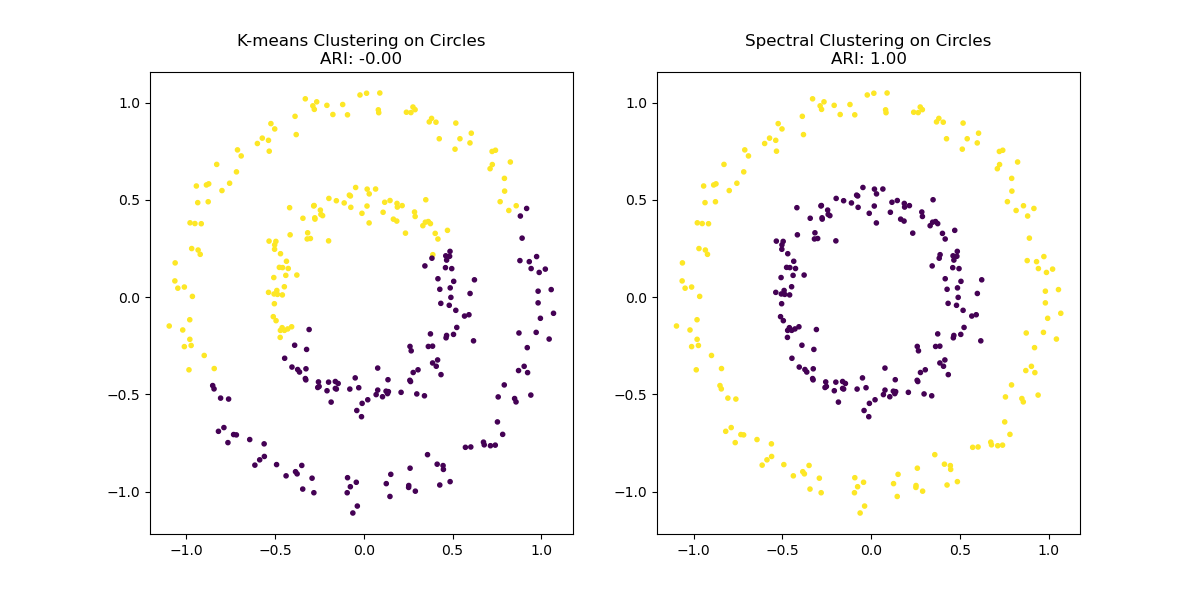
\includegraphics[scale=0.33]{circle.png} \label{1}
}
\quad
\subfigure[高斯数据]{
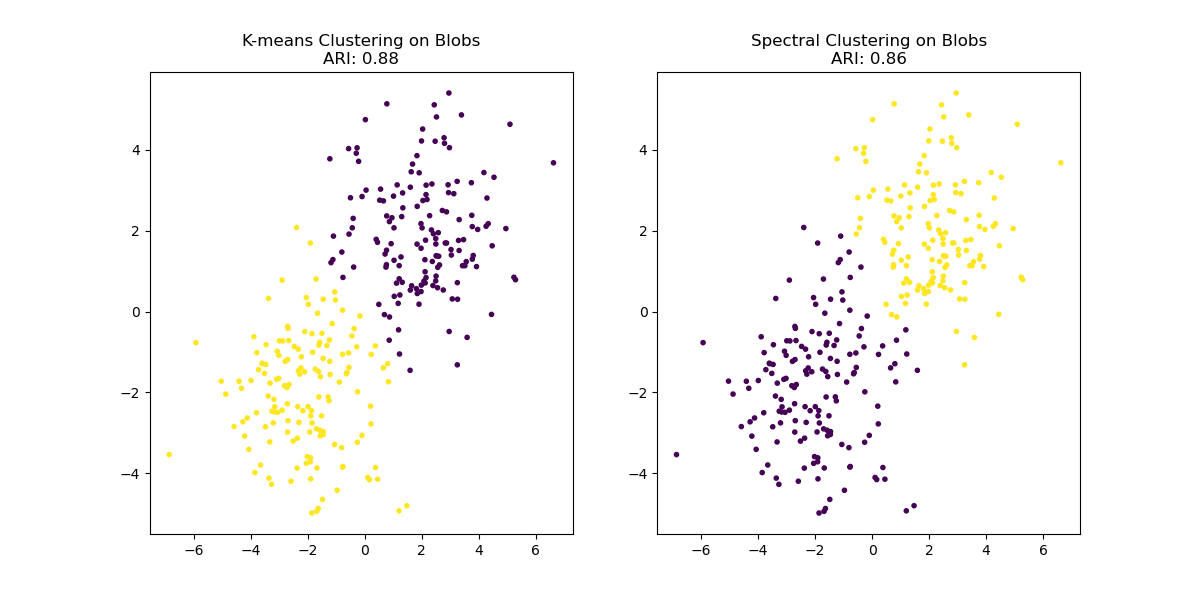
\includegraphics[scale=0.33]{guass_data.png} \label{2} 
}
\quad
\subfigure[半月形]{
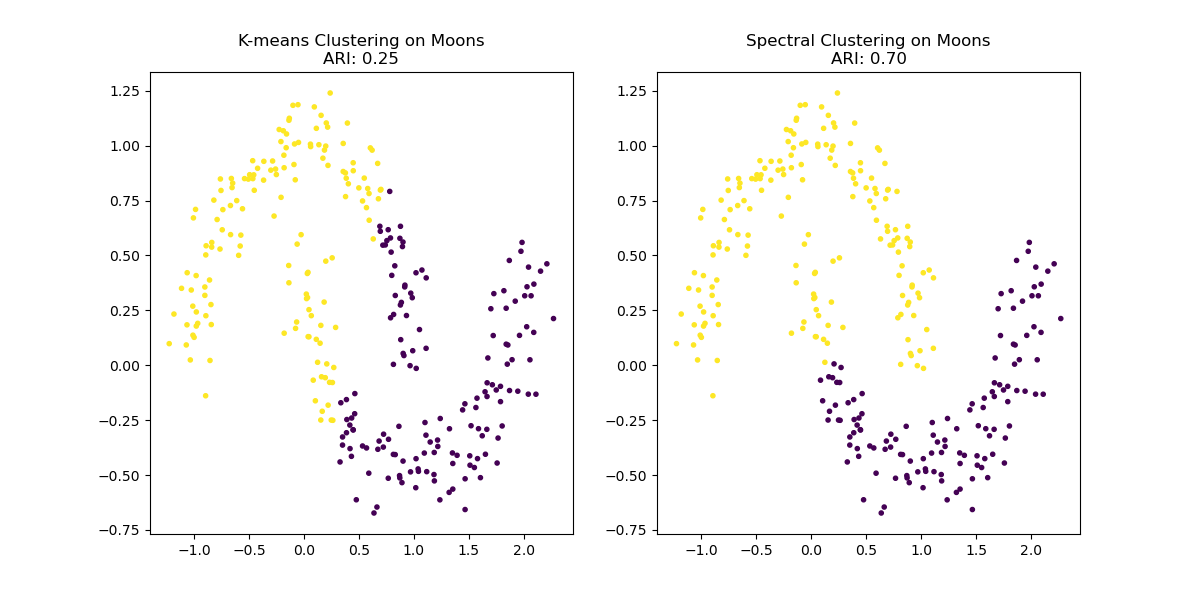
\includegraphics[scale=0.33]{semi_circle.png}\label{3}
}

\caption{谱聚类与k-means比较}
\end{figure}
结合图一分析,在接近凸形状的数据集(高斯混合)上,k-means和谱聚类都表现较好。k-means能够正确识别高斯分布的簇,而谱聚类的表现与k-means相当。\\
然而在两个非凸数据集(半月形和圆环)上,谱聚类明显优于k-means聚类。k-means无法正确识别非凸形状的簇,因为其假设簇的形状是凸的。这说明谱聚类通过图论方法,能够捕捉到数据的全局结构,适用于非线性和非凸的数据集,表现出更好的聚类效果。


\subsection{谱聚类对参数敏感性}
本小结将论证谱聚类的关键参数会极大程度上影响实验效果。我们通过构建邻接矩阵的构建方式($affinity$)和最邻近数($n\_neighbors$),并观察在非凸数据集(即两个半月形)上谱聚类的变化结果。同样我们利用$ARI$作为最终的评价指标。

\begin{figure}[htbp]
\centering
\subfigure[n=2]{
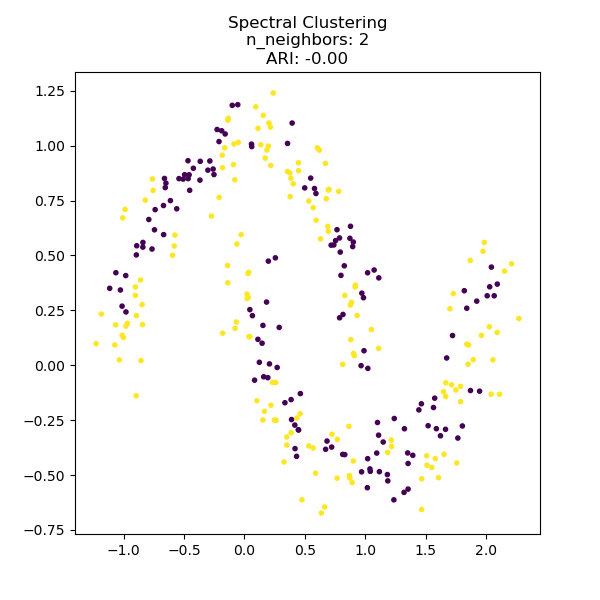
\includegraphics[scale=0.25]{n_2.png} \label{1}
}
\quad
\subfigure[n=5]{
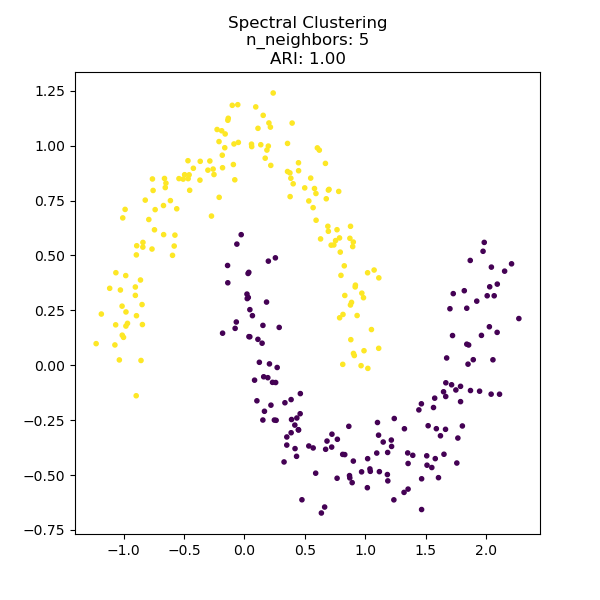
\includegraphics[scale=0.25]{n_5.png} \label{2} 
}
\quad
\subfigure[n=10]{
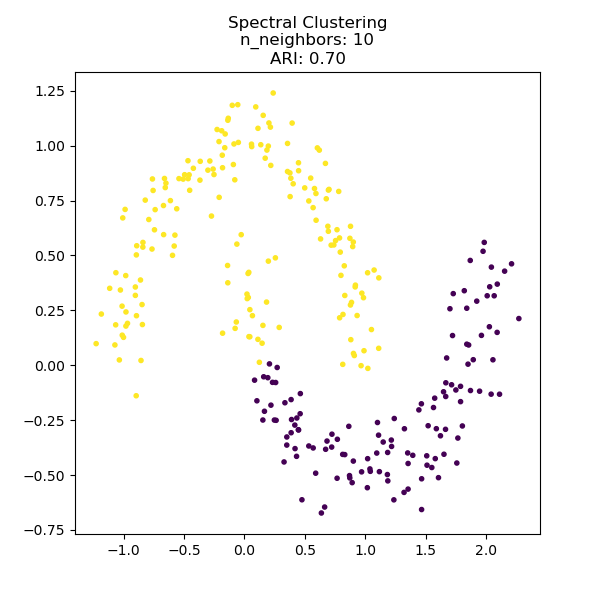
\includegraphics[scale=0.25]{n_10.png}\label{3}
}
\quad
\subfigure[n=20]{
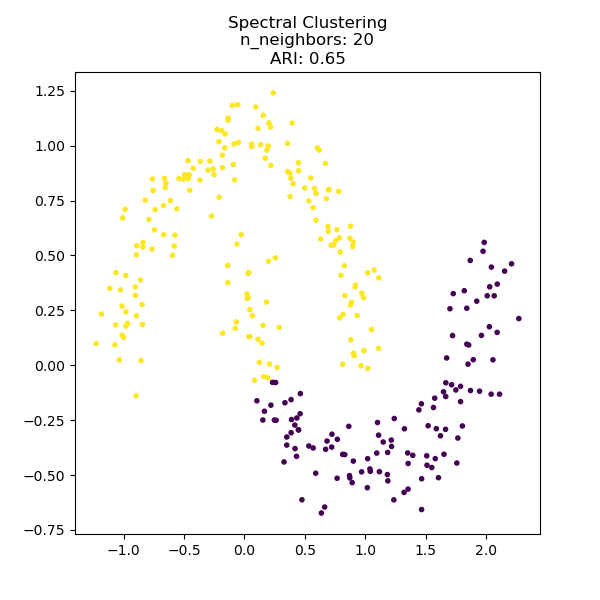
\includegraphics[scale=0.25]{n_20.png} \label{2} 
}
\caption{谱聚类对neighbors的敏感性}
\end{figure}
如图二所示,该实验说明,谱聚类对于参数$n\_neighbors$具有较高的敏感性。在$n\_neighbors=5$时,能够正确区分出两个半月形;而在$n\_neighbors=10,20$时,效果有所下降;在$n\_neighbors=2$时效果最差,完全无法进行区分。




\begin{figure}[htbp]
\centering
\subfigure[nearest]{
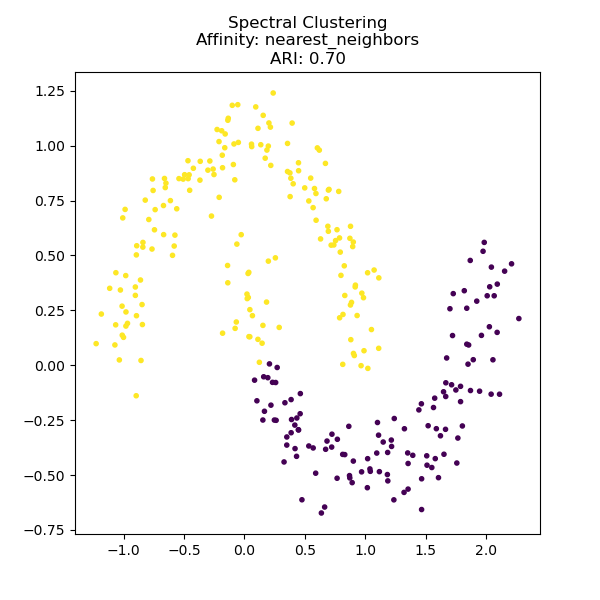
\includegraphics[scale=0.25]{nearest.png} \label{1}
}
\quad
\subfigure[rbf]{
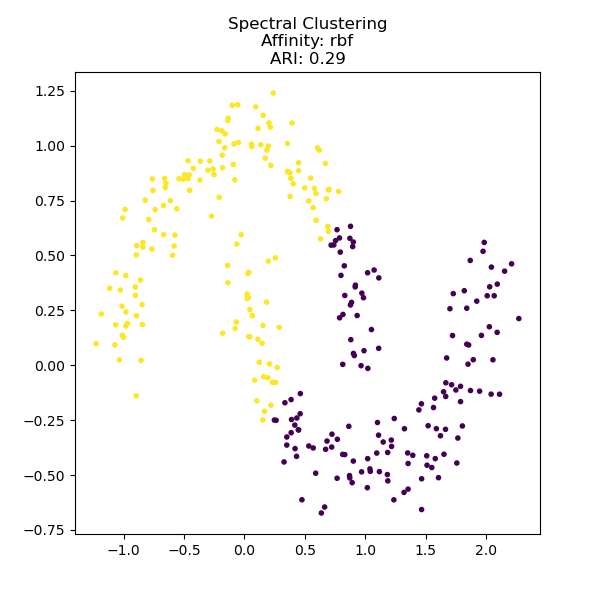
\includegraphics[scale=0.25]{rbf.png} \label{2} 
}
\caption{相似度矩阵构建方式对谱聚类影响}
\end{figure}
如图三所示,该实验对比利用$nearest\_neighbors$与$RBF$两种方式构建邻接矩阵,发现两个$ARI$差异较大。通过这个实验,可以观察到不同的相似度度量方式对谱聚类结果的影响。$nearest\_neighbors$通常适用于局部结构较强的数据集,而$RBF$适用于更复杂或全局结构重要的数据集。选择合适的相似度度量方式是使用谱聚类时的重要考虑因素,需要根据具体数据集的特点进行调整和优化。






\section{附录}
\subsection{拉普拉斯矩阵性质}
对于前文提及过的定理:拉普拉斯矩阵$L$有$n$个非负的特征值,并且$0\le \lambda_1\le...\le\lambda_n$,我们在这里给出详细的证明,并引申出一些更为深入的结论。首先我们对上述定理进行加强,得到如下两个定理:
\begin{theorem}
对于实对称矩阵$M$,以下三个论述等价:\\
$\bullet$ 存在矩阵$B$使得$M$可以分解为$B^TB$\\
$\bullet$ $M$是半正定矩阵\\
$\bullet$ $M$的所有特征值非负
\end{theorem}
这个定理可以让我们知道拉普拉斯矩阵$L$的所有特征值均非负,定理的证明如下

\begin{proof}
若$M=B^TB$,那么对于任意$x\in R^n$
$$
x^T M x=x^T BB^Tx=||B^Tx||^2_2\ge0\\
$$
若$M$为实对称矩阵,那么我们可以将$M$分解为
$$
M=RDR^T
$$
其中$D$为对角矩阵,且对角线元素为$M$的特征值,$R$为$M$的标准正交基构成的矩阵。
我们设$\vec{e_i}=(0,...,1,...,0)$为第$i$个$n$维的单位向量,并且令$x=R\vec{e_i}$,那么我们有
\begin{equation}
\begin{aligned}
0&\le x^T Mx\\
&=(R\vec{e_i})^TM(R\vec{e_i})\\
&=\vec{e_i}^T R^TRDR^T R \vec{e_i}\\
&=\vec{e_i}^T D \vec{e_i}\\ 
&=d_i
\end{aligned}
\end{equation}
因此$M$的所有特征值均非负。
若$M$的所有特征值非负,那么
$$
M=RDR^T=(D^\frac{1}{2}R)^T(D^\frac{1}{2}R)
$$
令$B=(D^\frac{1}{2}R)$即可

\end{proof}


\begin{theorem}
拉普拉斯矩阵$L$必有一个特征值为0
\end{theorem}

\begin{proof}
令$x\in R^n$并且各个维度均为1,那么
$$
Lx=(d_1-\sum_{i=1}^n w_{1i},...,d_n-\sum_{i=1}^n w_{ni})^T=\vec{0}
$$
\end{proof}


\begin{theorem}
拉普拉斯矩阵$L$中,特征值0的重数代表$L$对应的图$G$中连通分支的数量
\end{theorem}
由该定理可以推广得到一个结论,若$L$的特征值越接近于0,那么图$G$中会有一个子图$G'$,$G'$满足与$G$$\backslash$$G'$之间的边越少\\
个人认为该定理解释了利用拉普拉斯矩阵实现谱聚类的核心动机,这也说明谱分析的一个本质为即为用代数手段去解释图上的性质。\\
这里该定理的证明与我们的讨论主题实际相差较大,因此证明部分略去。




\section{参考文献}

\begin{thebibliography}{99}  
\bibitem{ref1}Nica, B. (n.d.). A Brief Introduction to Spectral Graph Theory. 瑞士: European Mathematical Society.
\bibitem{ref2}Cheverry, C., Raymond, N. (2021). A Guide to Spectral Theory: Applications and Exercises. 德國: Springer International Publishing.
\bibitem{ref3}Luxburg, U.V. (2007). A tutorial on spectral clustering. Statistics and Computing, 17, 395-416.
\bibitem{ref4}Andrew Y. Ng, Michael I. Jordan, and Yair Weiss. 2001. On spectral clustering: analysis and an algorithm. In Proceedings of the 14th International Conference on Neural Information Processing Systems: Natural and Synthetic (NIPS'01). MIT Press, Cambridge, MA, USA, 849–856.
\end{thebibliography}

\end{document}